%Nicht anfassen, so ist der Dokumentenaufbau
\documentclass[a4paper, 12pt]{article}
\usepackage{float}
\usepackage[T1]{fontenc} % Explizite Nennung des Fonts
\usepackage[utf8]{inputenc} % Kodierung
\usepackage{textcomp}
\usepackage[ngerman]{babel} % Sprache
\usepackage{graphicx} % immer benötigt für das Einbinden von Graphiken // hier egtl nicht mehr, wenn ledigilich eps.Dateien eingebunden werden...
\usepackage{blindtext} % Wenn man das Layout prüfen will, kann hier mit \blindtext Text eingfügt werden.
\usepackage{parskip} % Für den Abstand zwischen 2 Absätzen.
\setlength{\parskip}{12pt plus80pt minus10pt} % Genaue Einstellung von parskip
\usepackage{easy-todo} % Mit \todo{} Todos einfügen
\usepackage{csquotes} % Für ordentlichen Anführungszeichen
\usepackage[iso, german]{isodate} % Für eine deutsche Formatierung des Abgabedatums / Eidesstattlicher Erkärung
\usepackage[style=apa, backend=biber, sortlocale=de_DE]{biblatex}
% Biber backend für Literaturverzeichnis
\addbibresource{literatur/bibliography.bib} % Einbinden der Literatur.
\DeclareLanguageMapping{german}{german-apa} % Anpassen Spracheinstellungen im Literaturverzeichnis.
\usepackage[activate={true,nocompatibility},
	final,
	tracking=true,
	kerning=true,
	expansion=true,
	spacing=true,
	factor=1050,
	stretch=25,
	shrink=10]{microtype} % Für die Feineinstellung der Zeichensetzung.
\usepackage{booktabs} % Für Tabellen (toprule/midrule/bottomrule)
\usepackage{appendix} % Für den Anhang
\usepackage[rflt]{floatflt}
\usepackage{fancyvrb} % Für Styling
\usepackage[hidelinks]{hyperref} % Klickbare aber nicht markierte Links im PDF
\usepackage{setspace}
\usepackage[section]{placeins} %zwinge Tabellen und Abbildungen in das zugehörige Kapitel
\usepackage{fancyhdr} % Für schönere Kopf-/Fußzeilen und Fußnoten.
\usepackage[right=4 cm, left=2.5 cm, top=2.5 cm, bottom=3 cm]{geometry} % Seitenränder
\usepackage{pbox} % paragraphbox für multiline Tabellenzellen
\usepackage{tabulary} % Für Tabellen mit fixer Breite
\usepackage[nopostdot, nonumberlist, acronyms]{glossaries} % Für das Abkürzungsverzeichnis
\usepackage{listings} %Für das Einbinden von Code-Snippets im Anhang
\usepackage{float} % nötig für \restylefloat{table}
\restylefloat{table} % Für Tabellen an der exakten Position, wenn H als loc-param gegeben
\usepackage{longtable} %Für mehrseitige Tabelle

\makenoidxglossaries % Abkürzungsverzeichnis kompilieren
\renewcommand*{\glsnamefont}[1]{\textmd{#1}} % Abkürzungen weniger fett darstellen




\newacronym{acr}{ACR}{Awesome Acronym}






\glsaddall
\sloppy
\fancyhf{}
\rfoot{\thepage}
\renewcommand{\headrulewidth}{0pt}

%Special cells with linebreaks possible
\newcommand{\specialcell}[2][c]{%
	\begin{tabular}[#1]{@{}t@{}}#2\end{tabular}}
    
%define blockquote-quotation environment
\renewenvironment{quotation}{
	\leftskip1cm
	\rightskip1cm
	\noindent
	\setstretch{1}
	\small
}

% define Footnote
\renewcommand\footnoterule{\kern-3pt \hrule width 3in height 0.7pt \hskip3pt \kern 2.6pt}
\let\oldfootnote\footnote
\renewcommand\footnote[1]{%
	\oldfootnote{\hspace{2mm}#1}}
%%%%%

% microtyping around some characters

%Extra-spacing around dash, and quotation-marks, and parentheses
\SetExtraKerning[unit=space]
	{
		encoding={*}, family={qhv}, series={b}, size={normalsize,large,Large}
	}
	{
		\textendash={400,400}, % for double-dash
		\textquotedblleft={ ,120}, % for left quotation-mark
		\textquotedblright={170, }, % for right quotation-mark
		"28={ ,250}, % left bracket, add space from right
		"29={300, } % right bracket, add space from left
	}

%%%% Zeilenhöhe auf Microsoft Word anpassen.
\makeatletter
\newcommand{\MSonehalfspacing}{%
  \setstretch{1.44}%  default
  \ifcase \@ptsize \relax % 10pt
    \setstretch {1.448}%
  \or % 11pt
    \setstretch {1.399}%
  \or % 12pt
    \setstretch {1.433}%
  \fi
}
\newcommand{\MSdoublespacing}{%
  \setstretch {1.92}%  default
  \ifcase \@ptsize \relax % 10pt
    \setstretch {1.936}%
  \or % 11pt
    \setstretch {1.866}%
  \or % 12pt
    \setstretch {1.902}%
  \fi
}
\newcommand{\MSverbatimspacing}{%
  \setstretch{1.44}%  default
  \ifcase \@ptsize \relax % 10pt
    \setstretch {1}%
  \or % 11pt
    \setstretch {1}%
  \or % 12pt
    \setstretch {1}%
  \fi
}
\makeatother

%Acronyms
\newcommand*{\glossfirstformat}[1]{\textit{#1}}

\newacronymstyle{italic-on-first}
{%
  \GlsUseAcrEntryDispStyle{long-short}%
}%
{%
  \GlsUseAcrStyleDefs{long-short}%
  \renewcommand*{\genacrfullformat}[1]{%
   \glossfirstformat{\glsentrylong{##1}}\space
   (\glsentryshort{##1})%
  }%
  \renewcommand*{\Genacrfullformat}[2]{%
   \glossfirstformat{\Glsentrylong{##1}}\space
   (\glsentryshort{##1})%
  }%
  \renewcommand*{\genplacrfullformat}[2]{%
   \glossfirstformat{\glsentrylongpl{##1}}\space
   (\glsentryshortpl{##1})%
  }%
  \renewcommand*{\Genplacrfullformat}[2]{%
   \glossfirstformat{\Glsentrylongpl{##1}}\space
   (\glsentryshortpl{##1})%
  }%
}

\VerbatimFootnotes % von fancyvrb, erlaubt Syntax \footnote{\verb+verbatim+}

\newenvironment{changemargin}[2]{%
\begin{list}{}{%
\setlength{\topsep}{0pt}%
\setlength{\leftmargin}{#1}%
\setlength{\rightmargin}{#2}%
\setlength{\listparindent}{\parindent}%
\setlength{\itemindent}{\parindent}%
\setlength{\parsep}{\parskip}%
}%
\item[]}{\end{list}}
\begin{document}
\newgeometry{margin=2.5cm}
\begin{titlepage}
\thispagestyle{empty}
\newcommand{\HRule}{\rule{\linewidth}{0.5mm}}
\hspace{1cm}
\center

\textsc{\huge Universität Bremen}\\[2.0cm]
\textsc{\Large Fachbereich 08 - Soziologie}\\[0.8cm]
\MSonehalfspacing
\textsc{\Large Hausarbeit}\\[1.0cm]

\HRule\\[1.4cm]
\MSdoublespacing
{ \huge \bfseries Titel der Arbeit}\\[0.2cm]
{ \large Untertitel der Arbeit, falls gewünscht}\\[0.3cm] % Falls nicht benötigt, einfach auskommentieren
\HRule \\[2.4cm]
\MSonehalfspacing

\begin{minipage}[t]{0.8\textwidth}
	\begin{itemize}
	\item[\emph{VAK:}] Veranstaltungsnummer: VORNAME NAME des Dozenten
	\item[\emph{Semester:}] WiSe 2016/2017
	\item[\emph{Name:}] NACHNAME, VORNAME
	\item[\emph{Matr.-Nr.:}] 1234567
	\item[\emph{E-Mail:}] emailadresse@uni-bremen.de
	\item[\emph{Fachsemester:}] 03
	\item[\emph{Studiengang:}] MA[/BA] NAME DES STUDIENGANGS
	\end{itemize}
\end{minipage}

\vspace{2.9cm}

\flushright \emph{Abgabedatum:} \today
\end{titlepage}
\restoregeometry

\setstretch{3} % Zeilenabstand im Literaturverzeichnis hier anpassen
\microtypesetup{protrusion=false}
\tableofcontents
\microtypesetup{protrusion=true}
\thispagestyle{empty}

\MSonehalfspacing
\newpage
\setcounter{page}{1}
\pagestyle{fancy}


\setcounter{page}{1}
%%%%%%%%%%%%%%%%%%%%%%%%%%%%%
%%%Ab hier Inhalt einfügen%%%
%%%%%%%%%%%%%%%%%%%%%%%%%%%%%

\section{Einleitung} \label{einleitung}

Text der Einleitung

\section{Hauptteil}

Text des Hauptteils

\begin{figure}[htb]
\def\svgwidth{0.5\textwidth}
\fontsize{11}{8}\selectfont
\input{images/beispiel.eps_tex}
\end{figure}

.svg Dateien können mit dem freien Programm Inkscape in eps + eps\_tex umgewandelt werden. Speichern unter .eps -> 

\begin{figure}[H]
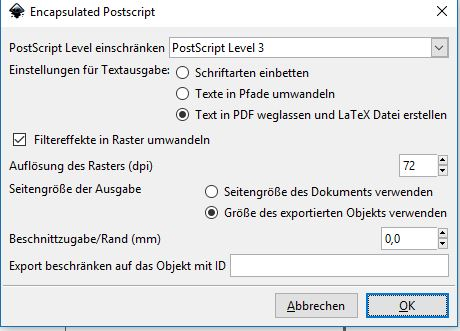
\includegraphics[width=\textwidth]{images/screenshot.jpg}
\caption{Mit diesen Einstellungen eps abspeichern}
\end{figure}

Gefährlich ist hier: Wenn die Vektorgraphiken nicht im Hauptverzeichnis abgelegt werden, muss der Pfad in Zeile 56 in der jeweiligen .eps\_tex - Datei angepasst werden.

Aus

\lstinline|\put(0,0){
\includegraphics[width=\unitlength]{beispiel.eps}}%|

muss

\lstinline|\put(0,0){
\includegraphics[width=\unitlength]{images/beispiel.eps}}%|

\subsection{Unterüberschrift 1}

Hier wird der Artikel von \textcite{Abadi.2016} zitiert \parencite{Abadi.2016}. Dabei kann man auch ein tolles \gls{acr} verwenden.

Der Anhang kann ich settings/endofdocument aktiviert werden.

\section{Schluss}

Das Abstract und alle Verzeichnisse zu Beginn des Dokuments werden am Ende von settings/titlepage verwaltet.

%%%%%%%%%%%%%%%%%%%%%%%%%%%%
%%%%%Ende des Dokuments%%%%%
%%%%%%%%%%%%%%%%%%%%%%%%%%%%
\newpage
\newpage


%\setlength\bibitemsep{\baselineskip}

\printbibliography
\newpage
%%Nicht anfassen, so ist der Dokumentenaufbau
\addtocontents{toc}{\protect\setcounter{tocdepth}{0}}
\renewcommand{\appendixtocname}{Anhang}
\addappheadtotoc
\renewcommand{\appendixpagename}{Anhang}
\appendices
\appendixpage
\appendixtitleoff
%%%%%%%%%%%%%%%%%%%%%%%%%%%%%
%%%Ab hier Inhalt einfügen%%%
%%%%%%%%%%%%%%%%%%%%%%%%%%%%%

% Anhang muss vorher für settings/endofdocument aktiviert werden.

%%%%%%%%%%%%%%%%%%%%%%%%%%%%
%%%%%Ende des Dokuments%%%%%
%%%%%%%%%%%%%%%%%%%%%%%%%%%%
\MSonehalfspacing
\restoreapp


\newpage
\section*{Eigenständigkeitserklärung}


Hiermit versichere ich, dass ich die Hausarbeit selbstständig verfasst und keine anderen als die angegebenen Quellen und Hilfsmittel benutzt habe, alle Ausführungen, die anderen Schriften wörtlich oder sinngemäß entnommen wurden, kenntlich gemacht sind und die Arbeit in gleicher oder ähnlicher Fassung noch nicht Bestandteil einer Studien- oder Prüfungsleistung war.

% 3,5cm Abstand nach oben
\vspace{100mm}
% Ort, Datum
\noindent{}STADT, den \today
% 8 cm breite Linie für die Unterschrift
\begin{minipage}[t]{8cm}
% gepunktete Linie
\centering \hspace{20mm} \hrulefill \\
% Text unter der Linie
\hspace{20mm}VORNAME NACHNAME
\end{minipage}
\end{document}